\documentclass[12pt,a4paper]{article}
\usepackage[utf8]{inputenc}
\usepackage[german]{babel}
\usepackage[T1]{fontenc}
\usepackage{amsmath}
\usepackage{amsfonts}
\usepackage{amssymb}
\usepackage{graphicx}
\usepackage{siunitx}
\usepackage{float}
\usepackage[left=2cm,right=2cm,top=2cm,bottom=2cm]{geometry}
\author{Tim}

\begin{document}
	\setlength{\parindent}{0pt} 
	\sisetup{separate-uncertainty = true}
	\begin{center}
		{\LARGE Versuchsprotokoll}\\
		\begin{large}
			zum Grundpraktikum Physik Teil II\\[0.4cm]
			an der RWTH Aachen\\
			I. Physikalisches Institut B\\[4.5cm]
			\Large\textbf{\textsl{Atomphysik}}\\[4cm]
			\normalsize\textit{vorgelegt\\von}\\[0.4cm]
			\large{Moritz Berger\\Tim Herbermann\\Gerald Kolter\\Sebastian Siebert}\\[1cm]
			\large \textit{Gruppe A07} \\ [3cm]
			\large \textbf{Sommersemester 2017}
		\end{large}
	\end{center}
	\newpage
	
\tableofcontents
\newpage

\section{Versuchsziele}
In diesem Versuch soll durch Vermessung der sogenannten Wärmestrahlung eines Lesliewürfels das Stefan-Boltzmann Gesetz nachgewiesen werden. Dabei sollen die Emissionskoeffizienten von 4 Seiten des Würfels bestimmt werden.

\section{Physikalische Grundlagen}
Jeder Körper hat eine Temperatur größer als \SI{0}{K} und sendet elektromagnetische Strahlung aus; diese wird Temperaturstrahlung oder auch Wärmestrahlung genannt. \\
Der Wärmeaustausch zwischen zwei Körpern kann auf 3 verschiedene Arten geschehen:
\begin{enumerate}
\item Konvektion: Der Austausch von Wärmeenergie durch Austausch von Teilchen
\item Wärmeleitung: Der Austausch von Wärmeenergie zwischen zwei einander berührende Körpern
\item Wärmestrahlung: Der Austausch von Wärmeenergie durch Abstrahlen von elektromagnetischer Strahlung bei einem der Körper und Absorption der Strahlung durch den anderen Körper
\end{enumerate}
Es soll in diesem Versuch nur um die Wärmestrahlung gehen, daher muss darauf geachtet werden, dass Konvektion und insbesondere Wärmeleitung verhindert wird. \\
Die Wärmestrahlung bildet ein kontinuierliches Spektrum. 

\paragraph{Das Plancksche Strahlungsgesetz}\mbox{}\\
Für das Emissionsvermögen eines schwarzen Körpers wurde um 1900 von Max Planck ein Modell vorgeschlagen, das die Quantenmechanik mitbegründet hat. Entscheidend hierbei ist, dass die elektromagnetische Wechselwirkung mit dem schwarzen Körper gequantelt ist; der Austausch von Energie mit dem Strahlungsfeld kann nur mit Vielfachen der Photonenenergie $E_\gamma = h \cdot f$ stattfinden. Für das Emissionsvermögen eines schwarzen Körpers ergibt sich das Plancksche Strahlungsgesetz zu:
\begin{equation}
E_{\lambda, s} = 2 \pi \cdot \dfrac{h c^2}{\lambda^5} \cdot \dfrac{1}{e^{\frac{hc}{\lambda kT}} - 1}
\end{equation}
Integriert man dieses Emissionsvermögen über alle Wellenlängen, erhält man die gesamte abgestrahlte Leistung:
\begin{equation}
P = E_s (T) = \int_0^\infty E_{\lambda, s} (\lambda, T) d\lambda = \sigma T^4 \qquad mit \qquad \sigma = \dfrac{2 \pi^5 k^4}{15h^3c^2}
\label{equ:Stefan_Boltzmann_Gesetz_schwarz}
\end{equation}
Für einen nicht-schwarzen Körper (also mit Emissionskoeffizient $\varepsilon \neq$ 1) muss Gl. \ref{equ:Stefan_Boltzmann_Gesetz_schwarz} modifiziert werden. Dabei werden in diesem Versuch zur Vereinfachung nur graue Körper betrachtet, das bedeutet, dass der Emissionskoeffizient $\varepsilon$ über die Wellenlänge konstant ist. Das Stefan-Boltzmann Gesetz sieht für solche Körper dann wie folgt aus:
\begin{equation}
P = \varepsilon \sigma T^4 \qquad mit \qquad \sigma = \dfrac{2 \pi^5 k^4}{15h^3c^2}
\label{equ:Stefan_Boltzmann_Gesetz_grau}
\end{equation}
Wichtig für die Auswertung ist, dass der Versuch in Luft bei Umgebungsdruck und Zimmertemperatur durchgeführt wurde. Die Umgebung strahlt ebenfalls auf den Körper, sodass die letztlich gemessene Strahlungsleistung die Differenz zwischen der Strahlung des Körpers und der Strahlung der Umgebung ist:
\begin{equation}
P = \varepsilon \sigma (T^4 - T_0^4)
\label{equ:Stefan_Boltzmann_Gesetz_gemessen}
\end{equation}
Mit der Umgebungstemperatur $T_0$.



\section{Aufbau und Durchführung}
\subsection{Aufbau}
\begin{figure}
\centering
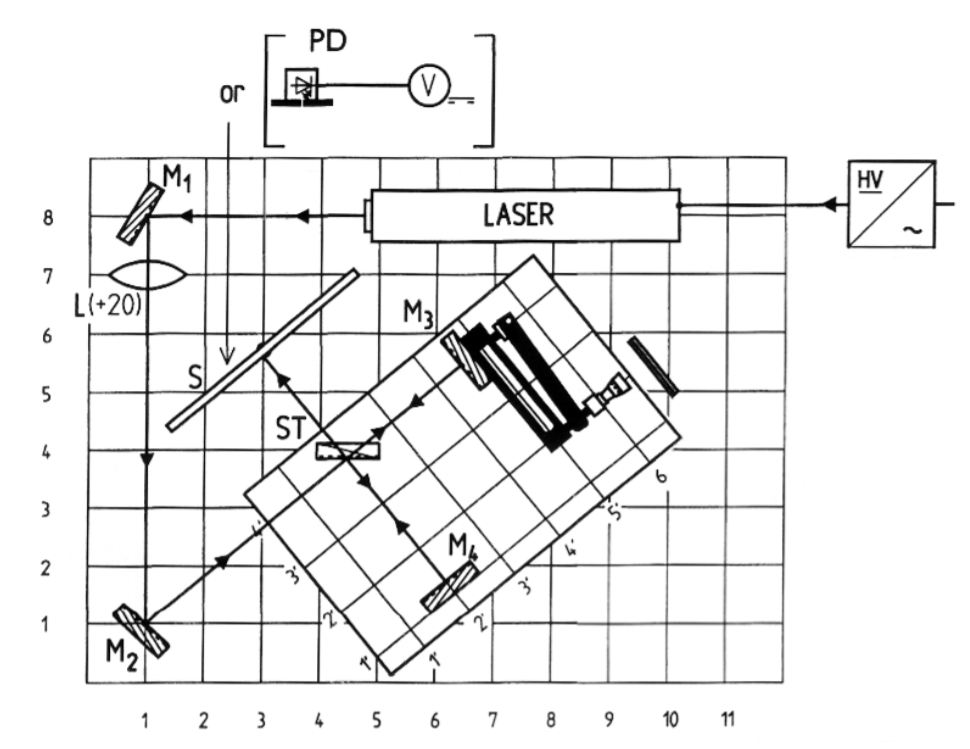
\includegraphics[scale=0.6]{Bilder/Aufbau.png}
\caption{Aufbau zur Vermessung der abgestrahlten Leistung einer der Seiten des Lesliewürfels. Die Nummerierung wird im Text erklärt.}
\label{fig:Aufbau}
\end{figure}

Abbildung \ref{fig:Aufbau} zeigt den Aufbau zur Vermessung der abgestrahlten Leistung einer der Seiten des Lesliewürfels.\\
Der Lesliewürfel (3) ist ein Würfel, der mit Wasser gefüllt auf einer Heizplatte (5) steht und 4 verschiedene Seiten hat. Zur besseren Wärmeverteilung im Wasser und damit im Würfel wird ein sogenannter Rührfisch verwendet; dies ist ein kleiner, stabförmiger Magnet, der von einem rotierenden Magneten unterhalb der Heizplatte gedreht wird und damit das Wasser umrührt. Die Temperatur des Wassers wird mit einem an das CASSY (6) angeschlossenen Thermometer gemessen. Die Strahlung wird mit einer Thermosäule nach Moll (2) gemessen. Diese befindet sich auf einer Schiene (1), die der Säule eine gewisse Stabilität gibt und erlaubt, die Thermosäule zwischendurch von dem Würfel zu entfernen, sodass sich das Schutzrohr nicht aufheizt. Da die Thermosäule nur sehr geringe Spannungen liefert, wird zwischen diese und das CASSY ein Verstärker (4) geschaltet.

\subsection{Durchführung}
Der Lesliewürfel wird mit Wasser befüllt und auf die Heizplatte gestellt und diese auf \SI{50}{\celsius} eingestellt. Während das Wasser sich erhitzt, wird mit dem Thermometer, mit dem später die Wassertemperatur gemessen wird, die Raumtemperatur gemessen und die Thermosäule auf die Wand gerichtet, um den Offset aus der Spannungsmessung raus zu nehmen, indem die Spannung durch setzen des Nullpunktes am Verstärker dort auf Null gesetzt wird. \\
Wenn der Würfel \SI{50}{\celsius} erreicht hat, wird die abgestrahlte Leistung vermessen. Dazu wird die Thermosäule wie in Abbildung \ref{fig:Aufbau} auf die Würfelseite gerichtet; dabei muss darauf geachtet werden, dass der Abstand zwischen Thermosäule und Würfel immer gleich eingestellt wird und dass die Thermosäule exakt senkrecht zur Würfelseite steht. Außerdem dürfen die Thermosäule und das Schutzrohr der Thermosäule den Würfel nicht berühren, da die in diesem Fall auftretende Wärmeleitung das Messergebnis verfälschen würde. Wenn sich die Spannung an der Thermosäule stabilisiert hat, wird die Messreihe gestartet. Anschließend wird der Würfel gedreht und die nächste Seite vermessen bis alle 4 Seiten vermessen wurden. Es ist sinnvoll, sich über die Reihenfolge Gedanken zu machen, denn wenn eine Seite mit hohem Emissionskoeffizienten gemessen wird, erhitzten sich die Thermosäule und das Schutzrohr dabei, sodass danach auf die Abkühlung gewartet werden müsste, wenn eine Seite mit niedrigerem Emissionskoeffizienten vermessen werden soll. Daher ist eine sinnvolle Reihenfolge, erst den Spiegel, dann die Messingseite, dann die weiße Seite und zum Schluss die schwarze Seite.\\
Nach der Vermessung aller 4 Seiten wird der Würfel um  \SI{5}{\celsius} weiter erhitzt und dabei die Thermosäule vom Würfel entfernt und wieder auf die Wand gerichtet, damit diese abkühlt. Anschließend werden die 4 Seiten erneut vermessen. Diese Vorgehensweise wird wiederholt bis das Wasser schließlich \SI{95}{\celsius} erreicht hat.\\
Da in diesem Versuch ein Thermometer verwendet wird, muss dieses noch kalibriert werden. Dazu werden mit dem Thermometer einmal Eiswasser und einmal siedendes Wasser gemessen.

\section{Auswertung}

\subsection{Kalibrierung}
Zunächst ist eine Kalibrierung des Thermometers notwendig. Dazu wird die Temperatur von Eiswasser und kochendem Wasser gemessen und gemäß des Zusammenhangs
 
\begin{equation}
T_{real} = a \cdot T_{Cassy} + b
\end{equation}

eine Kalibrierungsgerade durch die Punkte gelegt. Die gemessenen Referenzpunkte befinden sich in Tabelle \ref{tab:Kalibrierung}. Die ermittelten Parameter in Tabelle \ref{tab:Parameter}.

\begin{table}
\centering
\begin{tabular}{|c|c|c|}
\hline
Gruppe & A & B \\
\hline
Eis & \SI{273.56}{\K} & \\
\hline
Kochen & \SI{372.50}{\K} & \\
\hline 
\end{tabular}
\caption{Kalibrierungspunkte des Thermometers}
\label{tab:Kalibrierung}
\end{table}

\begin{table}
\centering
\begin{tabular}{|c|c|c|}
\hline
Gruppe & A & B \\
\hline
a & $1.0108$ & \\
\hline
b & \SI{-3.3551}{\K} & \\
\hline
\end{tabular}
\caption{Kalibrierungsparameter für Gruppe A und B.}
\label{tab:Parameter}
\end{table}

\subsection{Rohdaten}
\begin{figure}
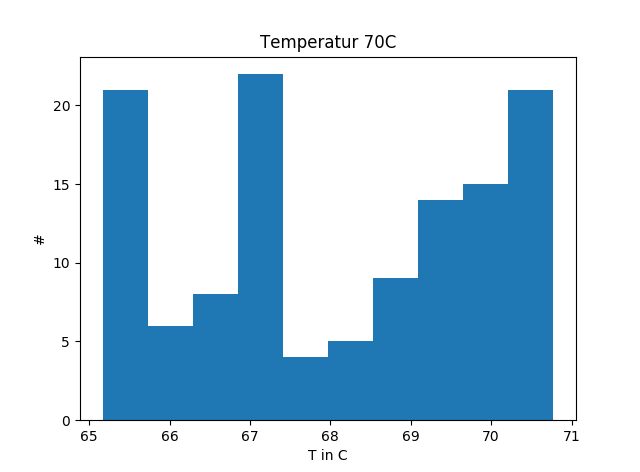
\includegraphics[scale=0.5]{Bilder/Rauschmessung_A_Temp.png}
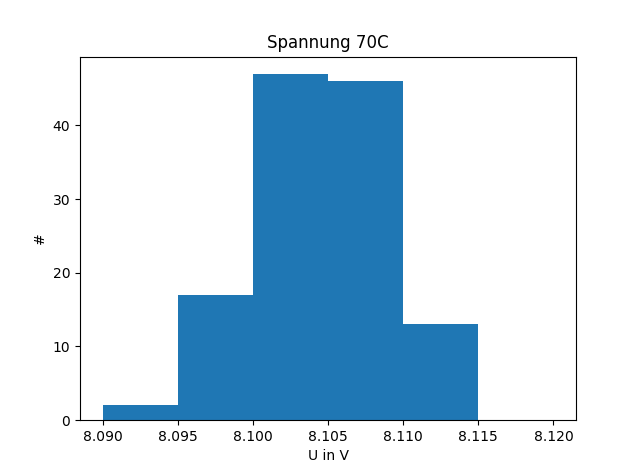
\includegraphics[scale=0.5]{Bilder/Rauschmessung_A_Spannung.png}
\caption{Rauschmessung von Gruppe A beispielhaft an der 70C Messung.}
\label{fig:Rausch_A}
\end{figure}

Bei jeder Messreihe wurden 125 Werte aufgezeichnet. Daraus wird der Mittelwert und der Fehler auf den Mittelwert bestimmt. In Abbildung \ref{fig:Rausch_A} und ??? sind diese Rauschmessung beispielhaft für beide Gruppen dargestellt. Die restlichen Rauschmessungen befinden sich im Anhang.\\
-Große Störung Temperatur\\


\subsection{Lineare Regressionen}
An den vorbereiteten Rohdaten werden nach Auftragung von $U$ gegen $T^4$ lineare Regressionen durchgeführt um den $T^4$ Zusammenhang des Stefan-Boltzmann-Gesetztes nachzuweisen. Dabei ist zu beachten, dass sich der Fehler auf den Mittelwert von $T$ gemäß 

\begin{equation}
\sigma_{T^4} = 4 \cdot T^3 \sigma_T
\end{equation}

fortpflanzt.

\begin{figure}[H]
\centering
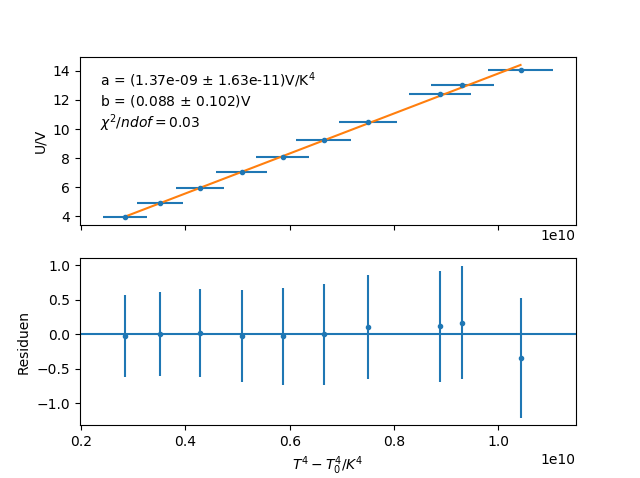
\includegraphics[scale=0.5]{Bilder/Schwarz_A}
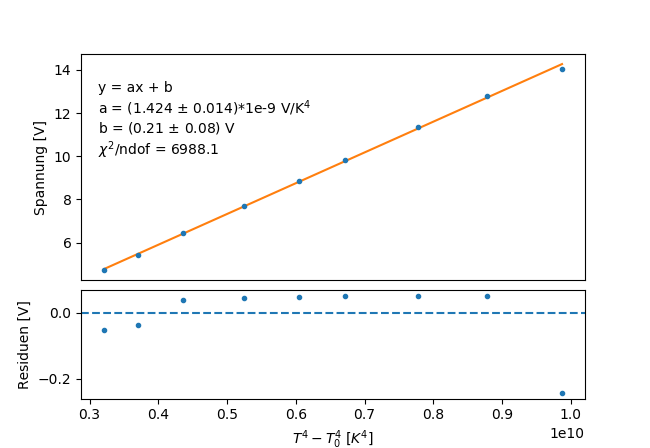
\includegraphics[scale=0.5]{Bilder/schwarz_B}
\caption{Lineare Regression an die Daten der schwarzen Seite. Gruppe A links und Gruppe B rechts.}
\label{fig:RegSchwarz}
\end{figure}

\begin{figure}[H]
\centering
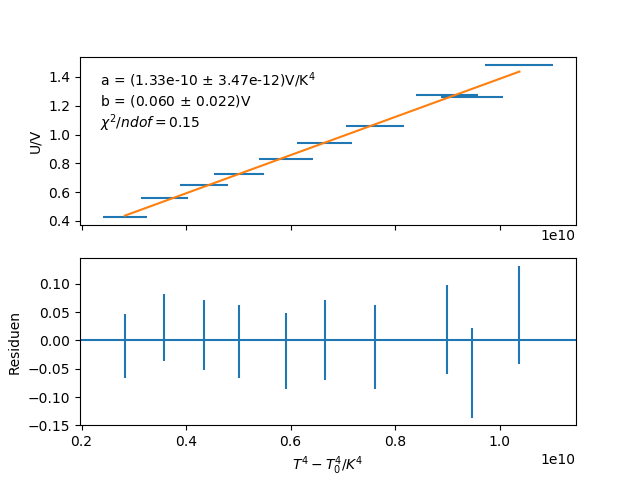
\includegraphics[scale=0.5]{Bilder/Weiss_A}
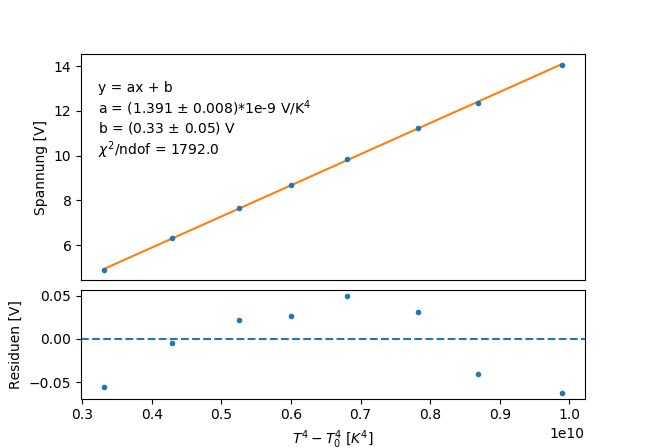
\includegraphics[scale=0.5]{Bilder/weiss_B}
\caption{Lineare Regression an die Daten der weißen Seite. Gruppe A links und Gruppe B rechts.}
\label{fig:RegWeiss}
\end{figure}

\begin{figure}[H]
\centering
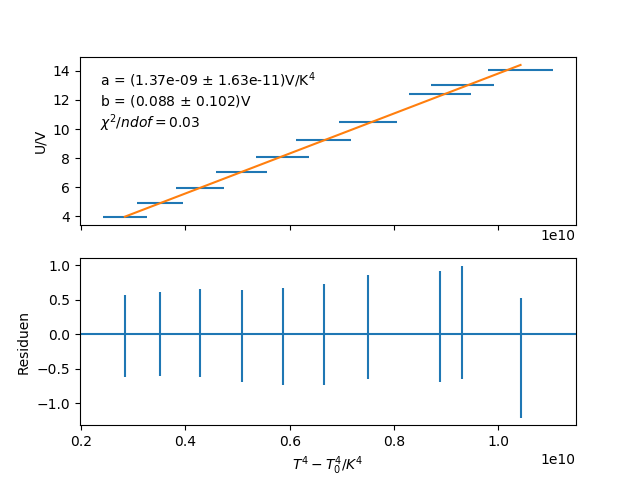
\includegraphics[scale=0.5]{Bilder/Messing_A}
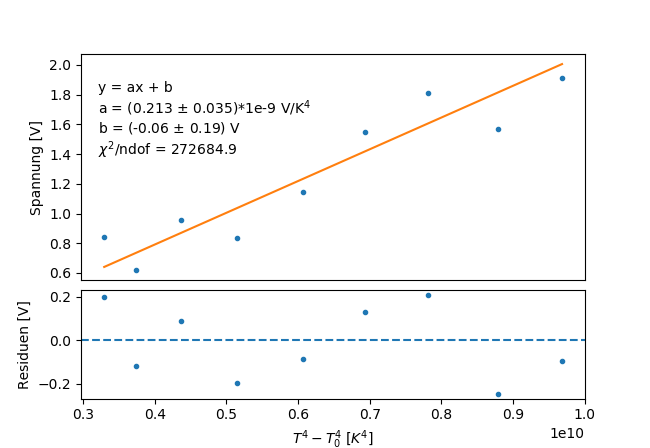
\includegraphics[scale=0.5]{Bilder/messing_B}
\caption{Lineare Regression an die Daten der messingfarbenen Seite. Gruppe A links und Gruppe B rechts.}
\label{fig:RegMessing}
\end{figure}

\begin{figure}[H]
\centering
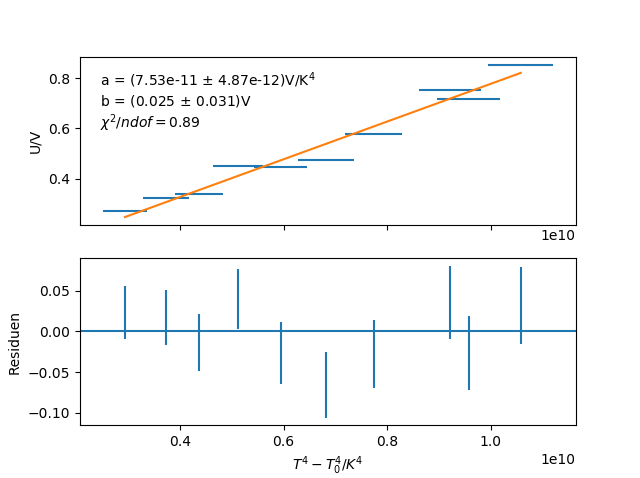
\includegraphics[scale=0.5]{Bilder/Spiegel_A}
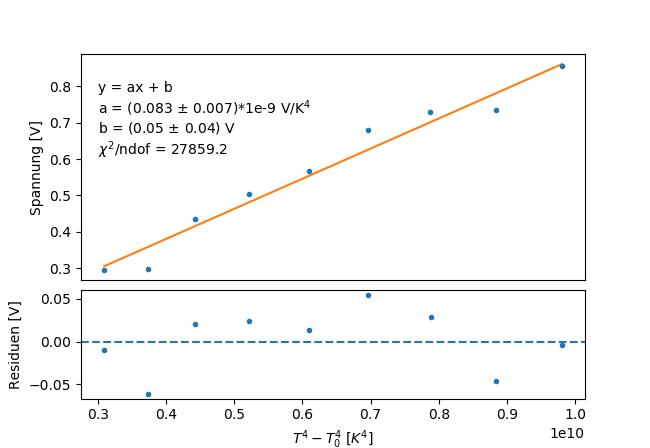
\includegraphics[scale=0.5]{Bilder/spiegel_B}
\caption{Lineare Regression an die Daten der spiegelnden Seite. Gruppe A links und Gruppe B rechts.}
\label{fig:RegSpiegel}
\end{figure}




\subsection{Emissionskoeffizient}

Für jede Seite des Würfels kann der Emissionskoeffizient bestimmt werden. Zusätzlich wird ein relatives $\epsilon_{rel}$, welches auf die bezüglich der schwarzen Seite normiert wurde, ermittelt um die Ergebnisse der beiden Gruppen besser vergleichen zu können.

Falls der y-Achsenabschnitt in den Anpassungen aus dem vorherigen Abschnitt im Rahmen seiner Fehler vernachlässigbar ist, könnte der Emissionskoeffizient in guter Näherung durch den Zusammenhang

\begin{equation}
\epsilon = \frac{P_{gemessen}}{P_{ideal}} = \frac{a v \pi r^2}{const A_s A_e \sigma}
\end{equation}

bestimmt werden. Falls der Abschnitt nicht vernachlässigbar wird 
der Koeffizient punktweise aus den Messwerten bestimmt. Der dazu nötige Zusammenhang lautet:

\begin{equation}
\epsilon = \frac{P_{gemessen}}{P_{ideal}} = \frac{U_{gemessen}vr^2 \pi}{const A_s A_e \sigma (T_{gemessen}^4-T_0^4)}
\end{equation}

Dabei bezeichnet $v = 10^{-4}$ den verwendeten Verstärkungsfaktor, $const$ die Empfindlichkeit der Thermosäule. $A_s = \pi \left(\frac{\SI{0,035}{\m}}{2}\right)$ und $A_e = \pi \left(\frac{\SI{0,023}{\m}}{2}\right)$, sowie $r = \SI{0,108}{\m}$ sind vorgegebene Konstanten in den Aufbauten beider Gruppen.\\

Für den statistischen Fehler auf $\epsilon$ gilt:

\begin{equation}
\sigma_{\epsilon, stat} = \epsilon \sqrt{ \left(\frac{\sigma_U}{U}\right)^2 + \left(\frac{4 \sigma_T}{T}\right)^2}
\end{equation}

und für den systematischen Fehler aus der Empfindlichkeit der Thermosäule:

\begin{equation}
\sigma_{\epsilon, sys} = \epsilon \frac{\sigma_{const}}{const}.
\end{equation}

Da nicht bei allen Anpassungen der Abschnitt im Rahmen seines Fehlers null war wurde der Emissionskoeffizient für bessere Vergleichbarkeit bei allen Seiten punktweise berechnet und anschließend gewichtet gemittelt.

Zudem wurden die Emissionskoeffizienten auf $\epsilon_{schwarz}$ normiert. Diese relativen Emissionskoeffizienten sind in Tabelle \ref{tab:Emission_relativ} angegeben:

\begin{equation}
\epsilon_{rel, i} = \frac{\epsilon_i}{\epsilon_{schwarz}}
\end{equation}

\begin{equation}
\sigma_{rel \,i, stat} = \frac{\sigma_{epsilon \,i}}{\epsilon_{schwarz}}
\end{equation}

\begin{equation}
\sigma_{rel \,i, sys} = \frac{\epsilon_{i}}{\epsilon_{schwarz}^2} \sqrt{\sigma_{schwarz, stat}^2 + \sigma_{schwarz, sys}^2}.
\end{equation}


\begin{table}
\centering
\begin{tabular}{|c|c|c|}
\hline
Gruppe & A & B \\
\hline
$\epsilon_{schwarz}$ & $ 0,979 \pm 0,011 \pm 0,030 $ & $ 0,856 \pm 0,001 \pm 0,026 $ \\
\hline
$\epsilon_{weiß}$ & $ 0,966 \pm 0,011 \pm 0,029 $ & $ 0,847 \pm 0,004 \pm 0,025 $ \\
\hline
$\epsilon_{Messing}$ & $ 0,101 \pm  0,001 \pm 0,003 $ & $ 0,129 \pm 0,005 \pm 0,004 $ \\
\hline
$\epsilon_{Spiegel}$ & $ 0,056 \pm 0,001 \pm 0,002 $ & $ 0,118 \pm 0,001 \pm 0,004 $ \\
\hline
\end{tabular}
\caption{Ermittelte Emissionskoeffizienten für beide Gruppen. Der Wert und der statistische Fehler ergeben sich durch Bildung des gewichteten Mittelwertes (innerer Fehler). Der systematische Fehler ist der relative Fehler der Empfindlichkeit, fortgepflanzt auf den Mittelwert von $ßepsilon$.}
\label{tab:Emission}
\end{table}

\begin{table}
\centering
\begin{tabular}{|c|c|c|}
\hline
Gruppe & A & B \\
\hline
$\epsilon_{rel,schwarz}$ & 1 & 1 \\
\hline
$\epsilon_{rel,weiss}$ & $ 0,987 \pm 0,011 \pm 0,061 $ & $ 0,988 \pm 0,004 \pm 0,296 $ \\
\hline
$\epsilon_{rel,Messing}$ & $ 0,103 \pm 0,001 \pm 0,006 $ & $ 0,151 \pm 0,006 \pm 0,011$ \\
\hline
$\epsilon_{rel,Spiegel}$ & $ 0,057 \pm 0,001 \pm 0,006 $ & $ 0,137 \pm 0,002 \pm 0,006$ \\
\hline
\end{tabular}
\caption{Auf $\epsilon_{schwarz}$ normierte Koeffizienten für beide Gruppen.}
\label{tab:Emission_relativ}
\end{table}



\subsection{Nicht-linearer Fit}
Anstelle eines linearen Fits zwischen der Spannung und der vierten Potenz der Temperatur kann auch eine Funktion der Form
\begin{equation*}
U = a + m \cdot T^n
\end{equation*}
an die Daten gefittet werden. Problem bei diesen nicht-linearen Fits ist häufig eine geringe Stabilität der Verfahren, sodass die Startwerte der Parameter mit Bedacht gewählt werden müssen. Hierbei bietet es sich an, die Parameter aus dem Ergebnis des linearen Fits zu verwenden. Aus dem Vergleich der angepassten Funktion mit der im linearen Fit bereits bestätigten Gl. \ref{equ:Stefan_Boltzmann_Gesetz_gemessen} ergeben sich die Startparameter zu:
\begin{equation*}
a = - \varepsilon \cdot \sigma \cdot T_0^4 \qquad m = \varepsilon \cdot \sigma \qquad n = 4
\end{equation*}

\begin{figure}
\centering
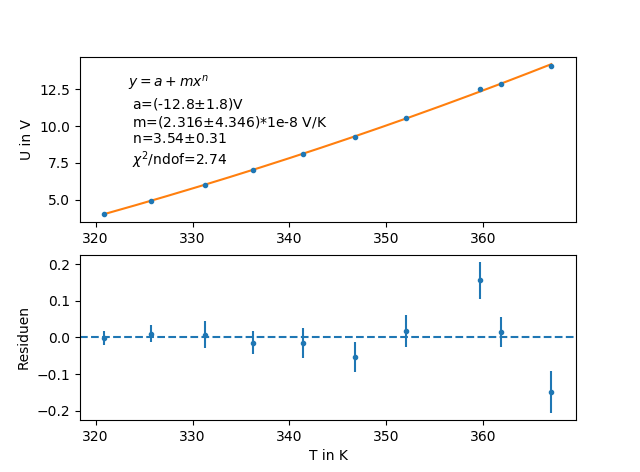
\includegraphics[scale=0.8]{Bilder/nichtlinear_A_weiss}
\caption{Nicht-lineare Regression an die Daten der weißen Seite.}
\label{fig:nicht_linearRegweiss_A}
\end{figure}

Abbildung \ref{fig:nicht_linearRegweiss_A} zeigt exemplarisch einen der nicht-linearen Fits.

\begin{table}
\centering
\begin{tabular}{|c|c|c|c|c|}
\hline
Messung & a $[V]$ & m $[\frac{V}{K^4}]$ & n & $\chi^2 / ndof$ \\
\hline
Messing Gruppe A & \num{-0.545(273)} & $(\num{2.860(177)}) \cdot 10^{-14}$ & \num{5.40(103)} & 61 \\
\hline
Spiegel Gruppe A & \num{0.0078(203)} & $(\num{2.890(149)}) \cdot 10^{-22}$ & \num{8.37(0)} & 192 \\
\hline
Weiß Gruppe A & \num{-12.8(18)} & $(\num{2.32(435)}) \cdot 10^{-8}$ & \num{3.540(307)} & 2.74 \\
\hline
Schwarz Gruppe A & \num{-13.80(379)} & $(\num{4.530(164)}) \cdot 10^{-8}$ & \num{3.43(59)} & 10.4 \\
\\
\hline
Messing Gruppe B & \num{-1.725(8003)} & $(\num{0.344(22804)}) \cdot 10^{-9}$ & \num{3.921(10886)} & 318275 \\
\hline
Spiegel Gruppe B & \num{-0.992(2964)} & $(\num{63.321(2177749)}) \cdot 10^{-9}$ & \num{2.916(5566)} & 29443.5 \\
\hline
Weiß Gruppe B & \num{-12.453(1149)} & $(\num{19.713(22989)}) \cdot 10^{-9}$ & \num{3.566(191)} & 590.9 \\
\hline
Schwarz Gruppe B & \num{-13.721(2835)} & $(\num{49.282(130796)}) \cdot 10^{-9}$ & \num{3.419(433)} & 4035.9 \\
\hline 
\end{tabular}
\caption{Ergebnisse der nicht-linearen Fits.}
\label{tab:Nicht_lin_Fit_Ergebnis}
\end{table}

Tabelle \ref{tab:Nicht_lin_Fit_Ergebnis} zeigt die Ergebnisse für die Parameter der nicht-linearen Fits. Anhand dieser und der Werte für das $\chi^2 / ndof$ lässt sich leicht erkennen, dass die meisten der nicht-linearen Fits nicht funktioniert haben. Erstaunlicherweise lässt sich beobachten, dass die meisten Werte für die Exponenten sehr nah am Erwartungswert dran sind.\\
Dennoch muss aufgrund der $\chi^2 / ndof$ und der geringen Stabilität des Verfahren gesagt werden, dass die Ergebnisse des nicht-linearen Fits keine Aussagekraft haben.


\section{Zusammenfassung}


\newpage
\section{Anhang}
\subsection{Rohdaten}
\subsubsection{Gruppe A}

\begin{figure}[H]
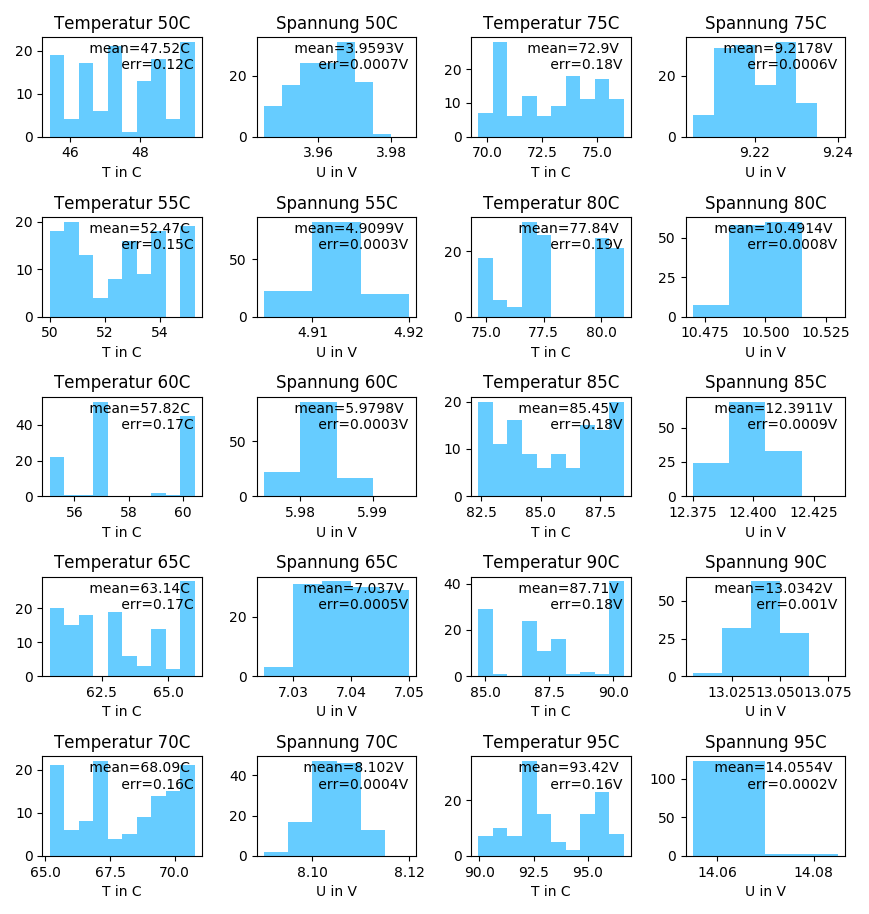
\includegraphics[scale=0.8]{Bilder/Rauschen_A_schwarz_2.png}
\caption{Rauschmessungen der schwarzen Seite von Gruppe A.}
\end{figure}

\begin{figure}[H]
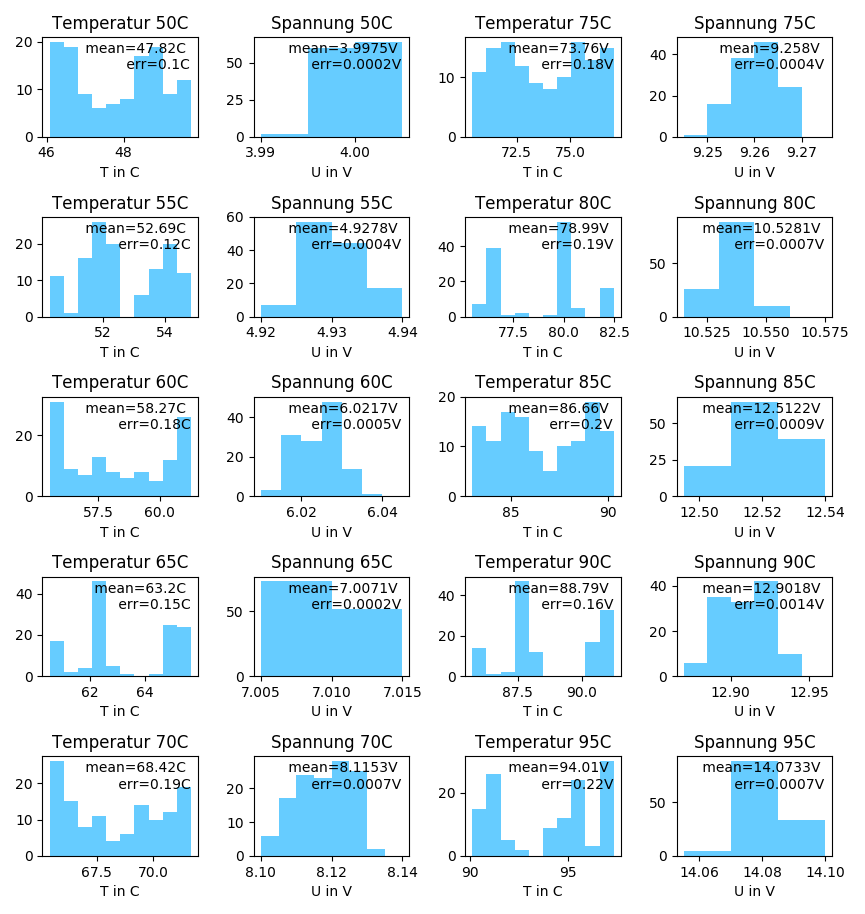
\includegraphics[scale=0.8]{Bilder/Rauschen_A_weiss_2.png}
\caption{Rauschmessungen der weißen Seite von Gruppe A.}
\end{figure}

\begin{figure}[H]
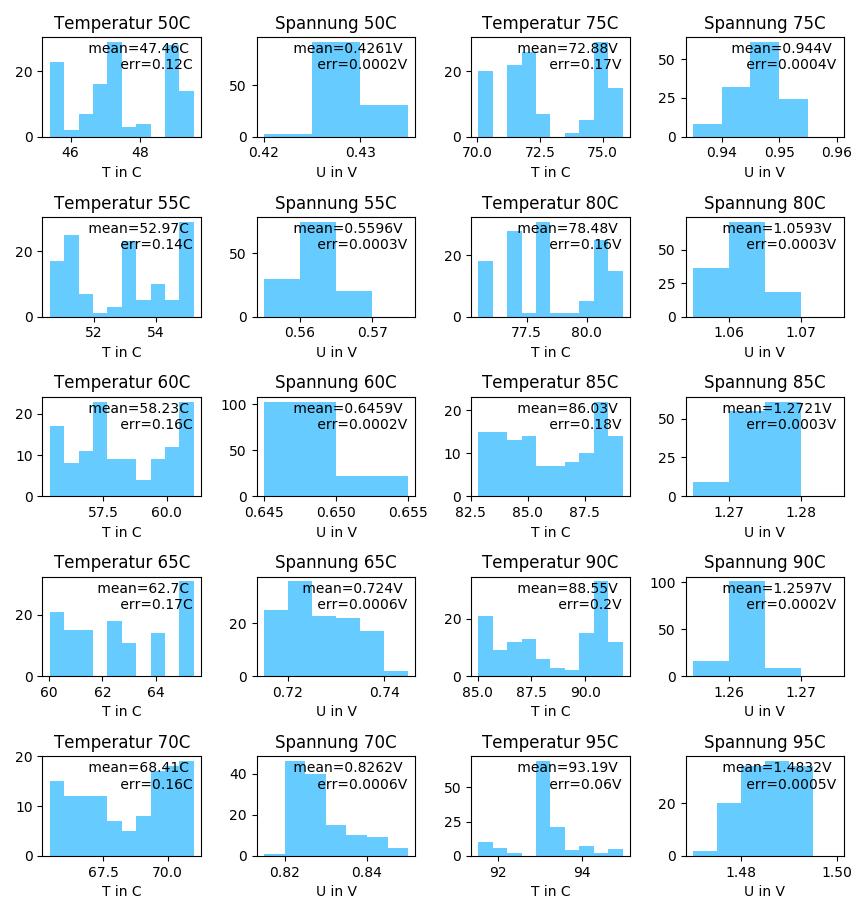
\includegraphics[scale=0.8]{Bilder/Rauschen_A_messing_2.png}
\caption{Rauschmessungen der Messing Seite von Gruppe A.}
\end{figure}

\begin{figure}[H]
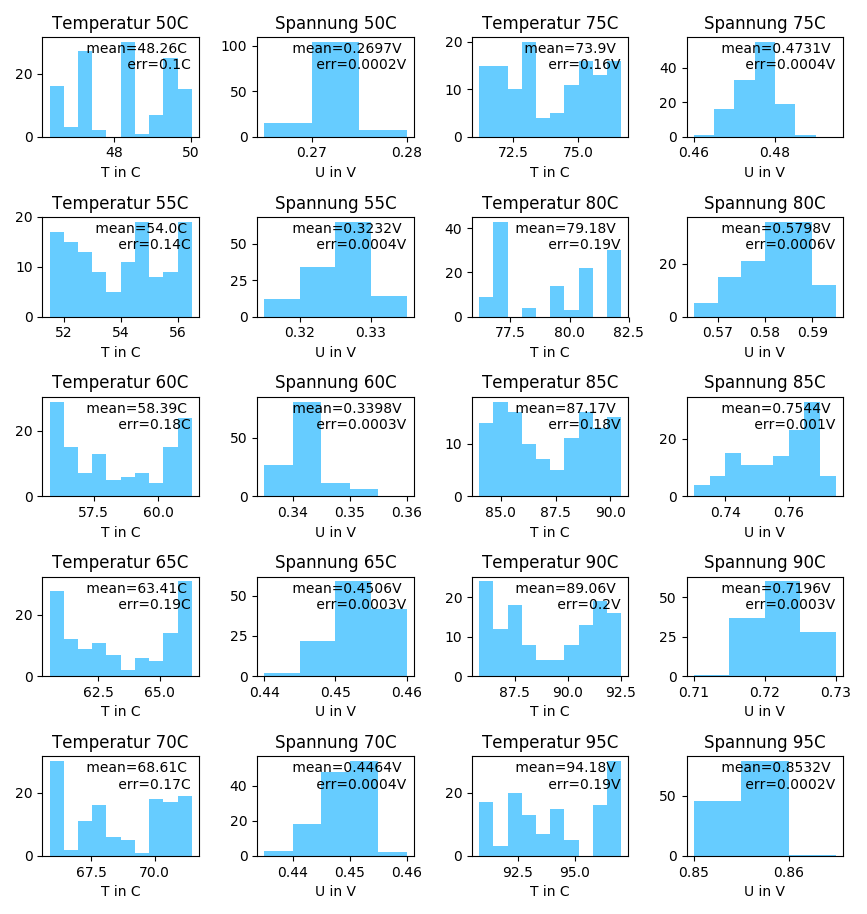
\includegraphics[scale=0.8]{Bilder/Rauschen_A_spiegel_2.png}
\caption{Rauschmessungen der spiegelnden Seite von Gruppe A.}
\end{figure}

\subsubsection{Gruppe B}

\begin{figure}[H]
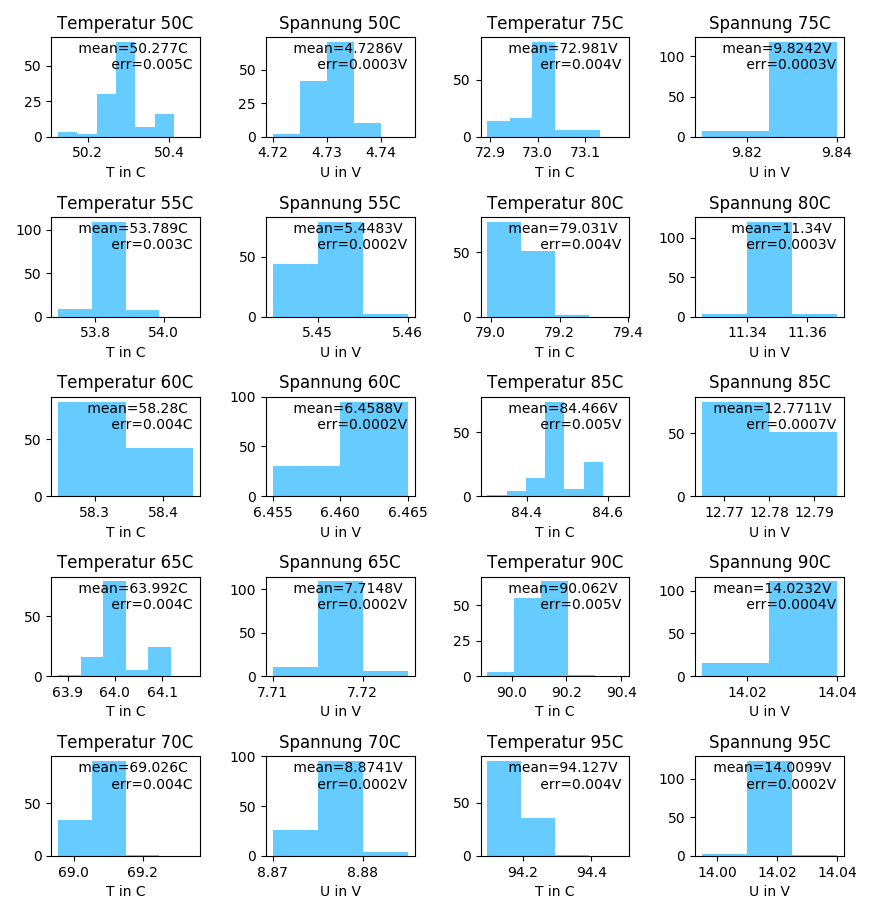
\includegraphics[scale=0.8]{Bilder/Rauschen_B_schwarz_2.png}
\caption{Rauschmessungen der schwarzen Seite von Gruppe A.}
\end{figure}

\begin{figure}[H]
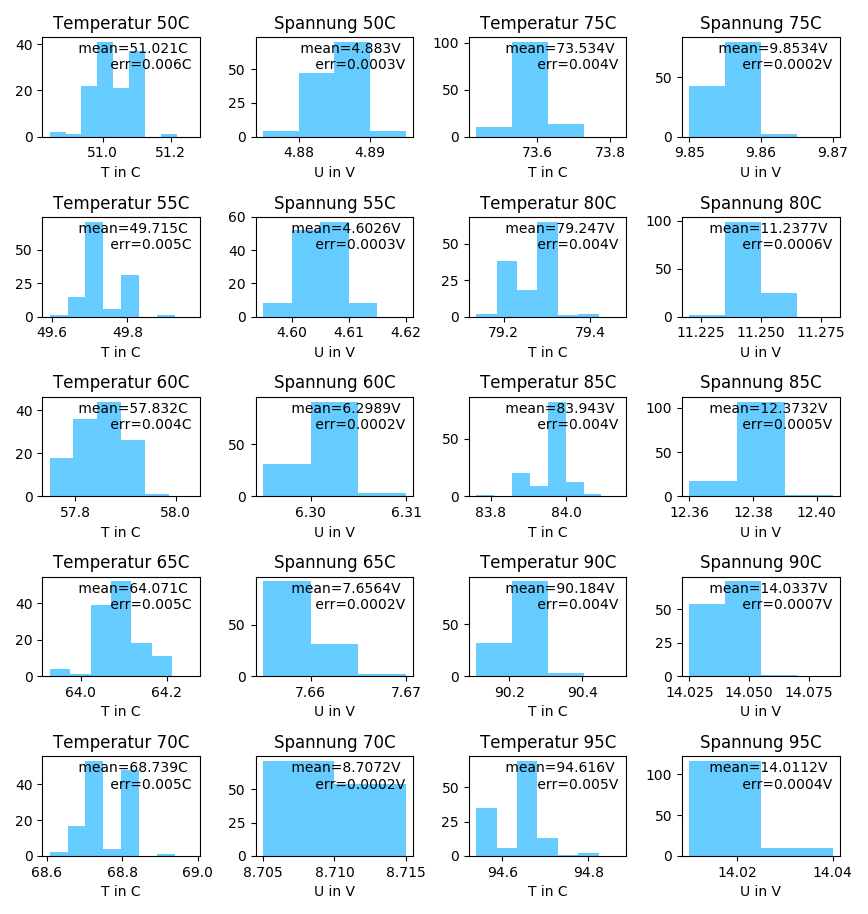
\includegraphics[scale=0.8]{Bilder/Rauschen_B_weiss_2.png}
\caption{Rauschmessungen der weißen Seite von Gruppe A.}
\end{figure}

\begin{figure}[H]
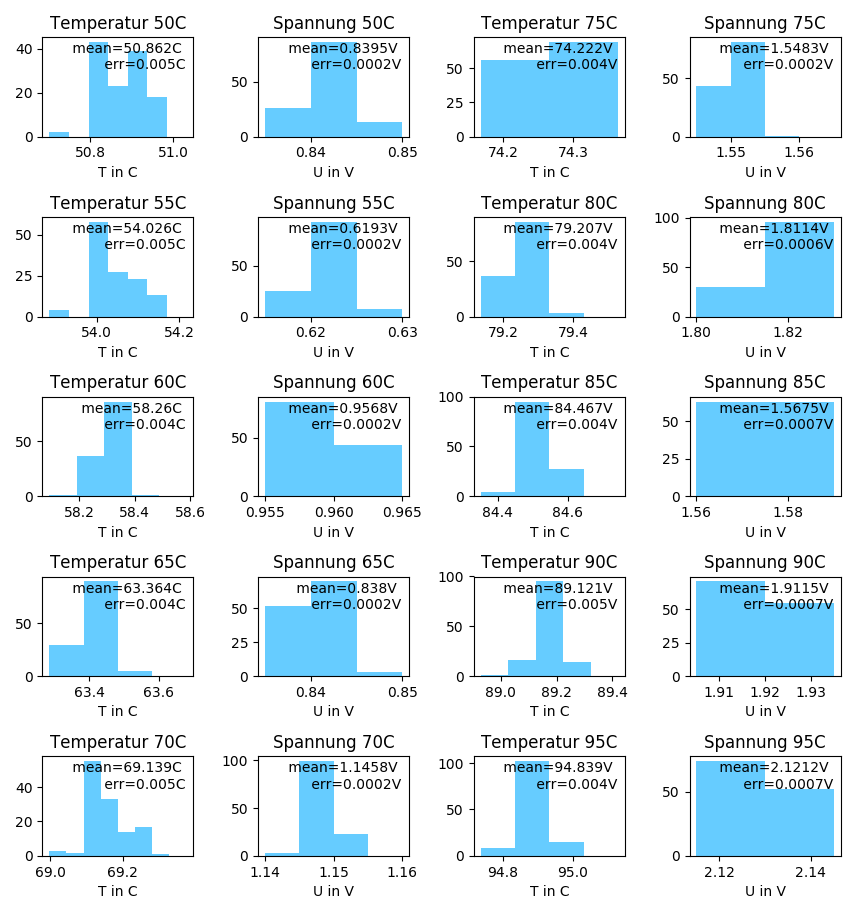
\includegraphics[scale=0.8]{Bilder/Rauschen_B_messing_2.png}
\caption{Rauschmessungen der Messing-Seite von Gruppe A.}
\end{figure}

\begin{figure}[H]
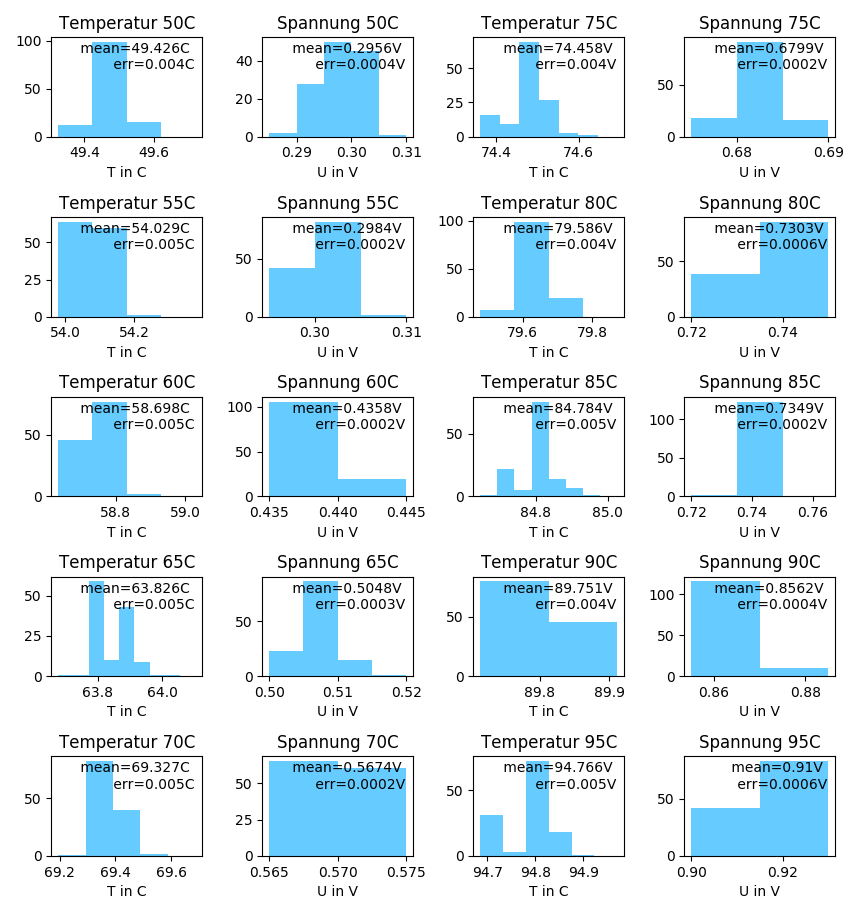
\includegraphics[scale=0.8]{Bilder/Rauschen_B_spiegel_2.png}
\caption{Rauschmessungen der spiegelnden Seite von Gruppe B.}
\end{figure}

\subsection{Nicht-linearer Fit}
\begin{figure}[H]
\centering
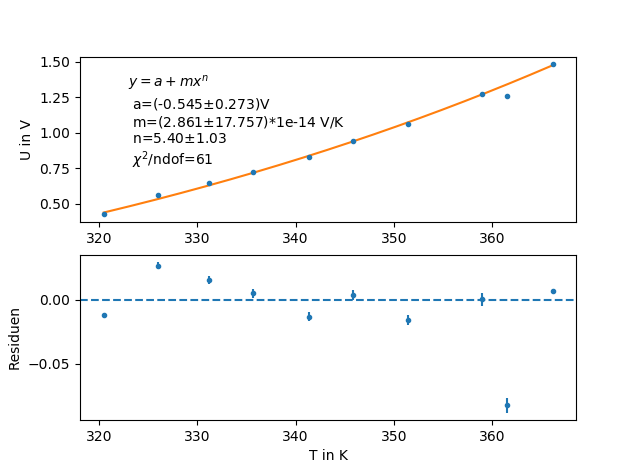
\includegraphics[scale=0.5]{Bilder/nichtlinear_A_messing.png}
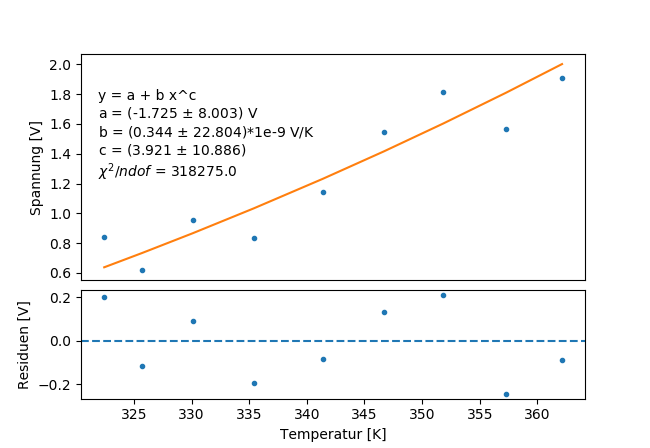
\includegraphics[scale=0.5]{Bilder/nonlinear_messing_B.png}
\caption{Nicht-linearer Fit an den Daten der Messing-Seite. Links der von Gruppe A, rechts der von Gruppe B.}
\end{figure}

\begin{figure}[H]
\centering
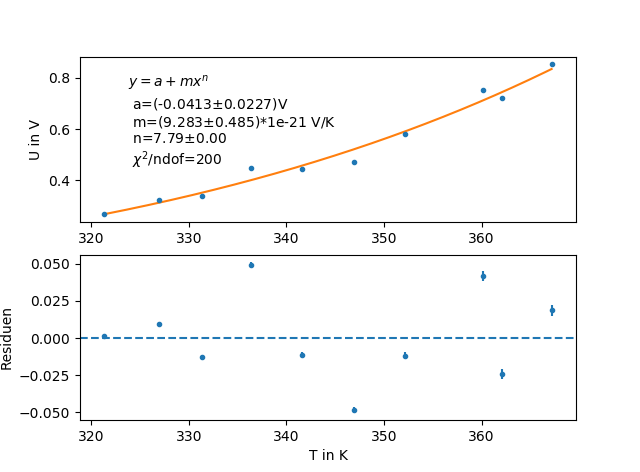
\includegraphics[scale=0.5]{Bilder/nichtlinear_A_spiegel.png}
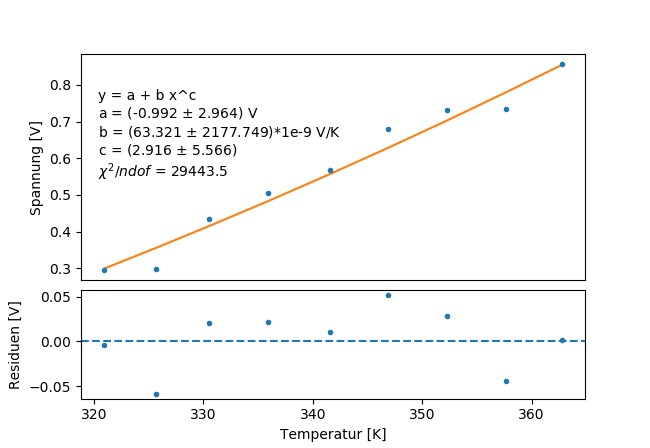
\includegraphics[scale=0.5]{Bilder/nonlinear_spiegel_B.png}
\caption{Nicht-linearer Fit an den Daten der Spiegel-Seite. Links der von Gruppe A, rechts der von Gruppe B}
\end{figure}

\begin{figure}[H]
\centering
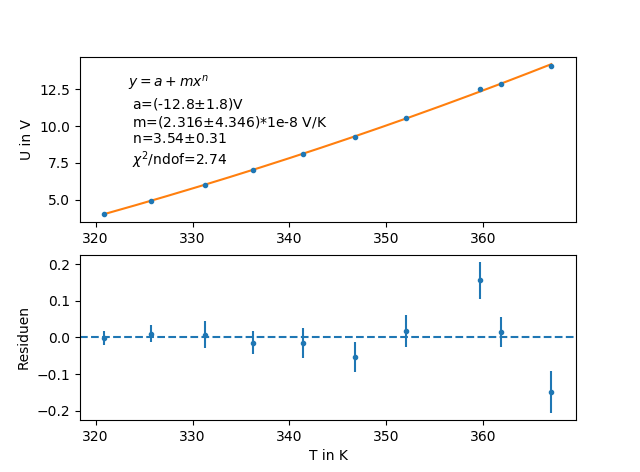
\includegraphics[scale=0.5]{Bilder/nichtlinear_A_weiss.png}
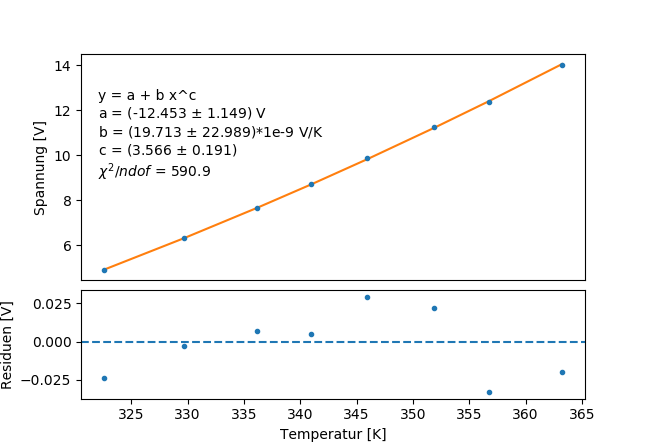
\includegraphics[scale=0.5]{Bilder/nonlinear_weiss_B.png}
\caption{Nicht-linearer Fit an den Daten der weißen Seite. Links der von Gruppe A, rechts der von Gruppe B.}
\end{figure}

\begin{figure}[H]
\centering
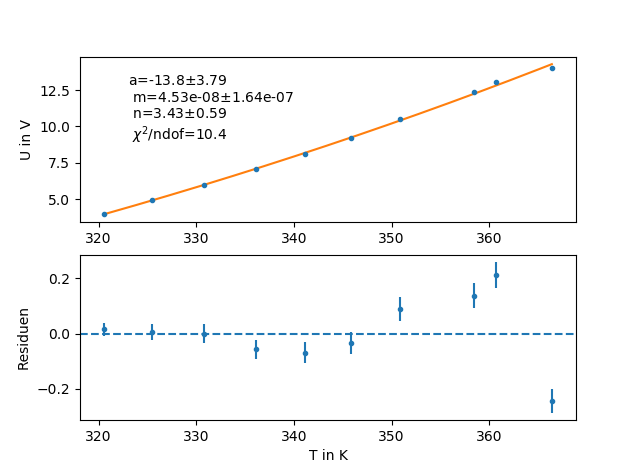
\includegraphics[scale=0.5]{Bilder/nichtlinear_A_schwarz.png}
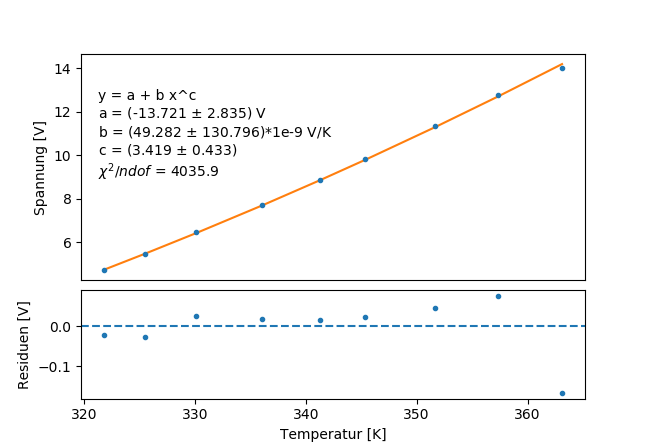
\includegraphics[scale=0.5]{Bilder/nonlinear_schwarz_B.png}
\caption{Nicht-linearer Fit an den Daten der schwarzen Seite. Links der von Gruppe A, rechts der von Gruppe B.}
\end{figure}
	
\end{document}